\documentclass[11pt,a4paper]{article}

% ------------------------------------------------------------------
%  Reporte - Reto Intelica: Forecasting de precios de berries con TDA
% ------------------------------------------------------------------
\usepackage[utf8]{inputenc}
\usepackage[T1]{fontenc}
\usepackage[margin=2.4cm]{geometry}
\usepackage{graphicx}
\usepackage{booktabs}
\usepackage{amsmath,amssymb}
\usepackage{siunitx}
\usepackage{float}
\usepackage{caption}
\usepackage{subcaption}
\usepackage{enumitem}
\usepackage[hidelinks]{hyperref}

\graphicspath{{figures/}}
\captionsetup{font=small,labelfont=bf}

% Nombres en español (sin babel-spanish instalado)
\renewcommand{\figurename}{Figura}
\renewcommand{\tablename}{Tabla}
\renewcommand{\abstractname}{Resumen}
\renewcommand{\refname}{Referencias}

\title{Forecasting del precio de berries (WPUSI01102B):\\
comparación de modelos con y sin Análisis Topológico de Datos (TDA)}
\author{Diana Laura Hernández Almeida \and Gonzalo Makenly Higuera Inzunza \and
José Alfredo López Torres \and Juan Pablo de la Peña Gonzalez \and
Sarah Camila Guzmán Fierro \\[0.5em] Reto Intelica --- Proyecto berry-price-tda}
\date{Junio de 2026}

\begin{document}
\maketitle

\begin{abstract}
\noindent
Este trabajo estudia la predicción mensual del índice de precios al productor
de berries en EE.\,UU. (serie WPUSI01102B de FRED). El objetivo central es
determinar si las características derivadas del Análisis Topológico de Datos
(TDA), es decir la homología persistente sobre embeddings de Takens de la serie,
mejoran de forma estadísticamente significativa el desempeño de modelos de
forecasting respecto a sus equivalentes sin TDA. Para ello se diseñó un
experimento factorial de gran escala (cerca de 19\,200 combinaciones de modelo,
ventana, transformación, exógenas, estrategia de anomalías y uso de TDA),
evaluado con validación cruzada temporal, y se contrastó con un conjunto de
prueba fijo intacto (2022 en adelante). Los resultados muestran que el efecto del
TDA es estadísticamente detectable pero de magnitud insignificante
($\delta$ de Cliff $=0.047$) y, de hecho, ligeramente desfavorable en MAE; el
mejor modelo final es un Ridge sin TDA ni exógenas (MAE $=29.79$). Se concluye
que, para esta serie, la topología no aporta señal predictiva útil más allá de la
ya contenida en los retardos.
\end{abstract}

% ==================================================================
\section{Introducción}
% ==================================================================

\subsection{Descripción del problema}
Los precios de las berries (fresas, arándanos, frambuesas) son notoriamente
volátiles: combinan una marcada estacionalidad anual (ligada a ciclos de
cosecha), tendencias de mediano plazo (inflación, costos de insumos) y choques
abruptos (clima, logística). Predecir su evolución es relevante para
productores, comercializadores y planeación de inventarios. Trabajamos sobre el
Producer Price Index de berries de la Bureau of Labor Statistics de EE.\,UU.,
publicado por FRED bajo el identificador WPUSI01102B, una serie mensual con
fuerte componente estacional y no estacionaria en nivel.

\subsection{Objetivo}
El objetivo del estudio es comparar modelos de forecasting con y sin TDA para el
horizonte $t{+}1$ (y proyecciones a futuro), respondiendo de forma cuantitativa
y con pruebas de hipótesis a tres preguntas:
\begin{enumerate}[noitemsep]
  \item ¿El uso de características topológicas (TDA) mejora la precisión de
        forma estadísticamente significativa?
  \item ¿El uso de variables exógenas la mejora?
  \item ¿Qué factores del pipeline (modelo, ventana, transformación) influyen
        más en el error?
\end{enumerate}

\subsection{Datos}
La serie objetivo WPUSI01102B se descarga directamente de FRED
(script download\_berry\_data.py) y abarca 215 observaciones mensuales desde
junio de 2008 hasta abril de 2026. El índice varía entre $69.2$ y $299.4$, con
media cercana a $142.5$.

Adicionalmente se construyó un conjunto de variables exógenas
(script download\_exogenous.py), alineadas a frecuencia mensual:
\begin{itemize}[noitemsep]
  \item cpi\_fresh\_fruits: CPI de frutas frescas (FRED CUSR0000SAF113), presión de demanda.
  \item ppi\_fertilizers: PPI de fertilizantes (FRED WPU0652), costo de insumos.
  \item diesel\_price: precio del diésel USD/galón (FRED APU000074714), costo logístico.
  \item mxn\_usd: tipo de cambio FIX MXN/USD (Banxico SF43718), relevante por el origen de importaciones.
\end{itemize}
Las series se consolidan en data/interim/berry\_features.csv, con imputación
conservadora (forward y backward fill) de huecos puntuales. La
Figura~\ref{fig:serie} muestra la serie completa.

\begin{figure}[H]
  \centering
  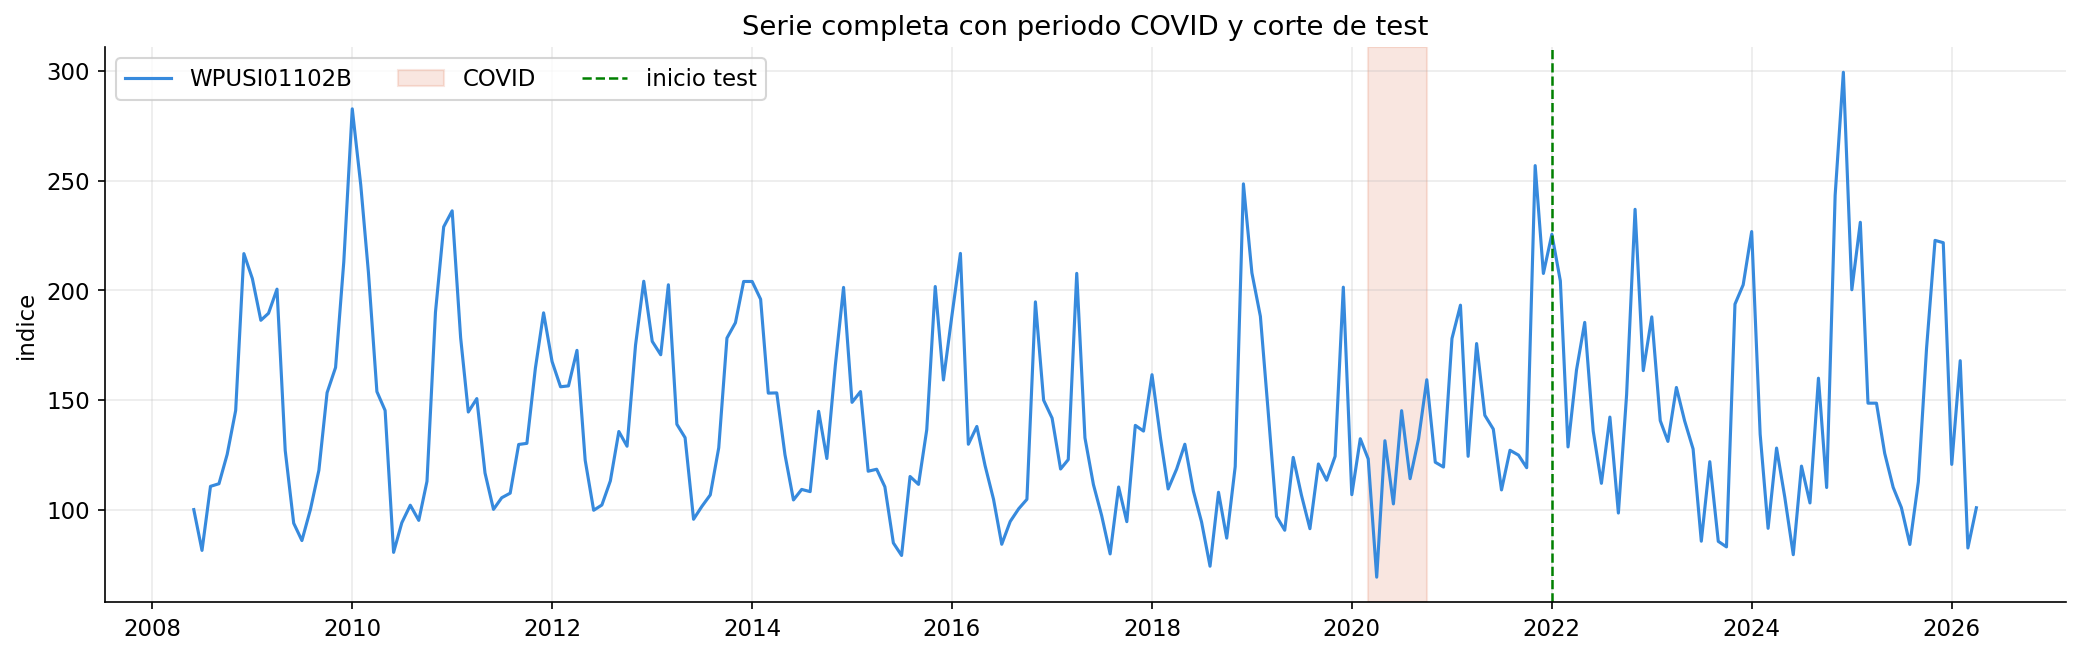
\includegraphics[width=0.9\textwidth]{fig_serie_completa.png}
  \caption{Serie histórica del índice WPUSI01102B (2008 a 2026), con su marcada
  estacionalidad anual, tendencia creciente y choques de precio.}
  \label{fig:serie}
\end{figure}

% ==================================================================
\section{Metodología}
% ==================================================================

\subsection{Análisis Topológico de Datos (TDA) en series de tiempo}
El TDA cuantifica la forma de los datos. Para una serie temporal 1D se aplica el
siguiente pipeline por ventana (módulo features/tda.py):
\begin{enumerate}[noitemsep]
  \item Embedding de Takens: cada ventana 1D se transforma en una nube de puntos
        en $\mathbb{R}^d$ mediante retardos (dimensión de embedding $=6$,
        time delay configurable). Si la serie tiene dinámica periódica, esta nube
        traza un lazo.
  \item Homología persistente (Vietoris--Rips) sobre la nube, que detecta
        componentes conexas ($H_0$) y ciclos o lazos ($H_1$) a múltiples escalas.
  \item Diagrama de persistencia $(\text{birth},\text{death})$ de los rasgos
        topológicos.
  \item Vectorización en 8 características por ventana: max\_pers\_h1,
        mean\_pers\_h1, std\_pers\_h1, n\_cycles\_h1, entropy\_h1 (entropía de
        persistencia), amplitude\_h1 (norma $L_2$), max\_pers\_h0 y n\_comp\_h0.
\end{enumerate}
La intuición es que la persistencia de los ciclos $H_1$ codifica la fuerza de la
estacionalidad de cada ventana de forma invariante a traslaciones y
deformaciones suaves. Las matrices TDA se sanean (eliminación de columnas
constantes y recorte de valores extremos a $\pm 5\sigma$ con estadísticos del
entrenamiento) para no desestabilizar a los modelos lineales.

\subsection{Pipeline con y sin TDA}
El problema se plantea como regresión supervisada a un paso (features/builder.py):
mediante ventanas deslizantes de tamaño $w$ se construye $X$ y se predice el
valor en $t{+}1$. La matriz de diseño ensambla bloques de forma factorial:
\begin{itemize}[noitemsep]
  \item Retardos del objetivo (la ventana), siempre presentes.
  \item Exógenas (valor actual con retardos opcionales), de manera opcional.
  \item Características TDA de la ventana, opcional, que es el factor en estudio.
\end{itemize}
Para combatir la no estacionariedad el objetivo se modela en transformación
(none, standard, diff, log\_diff, seasonal\_diff); el nivel se reconstruye
después sumando la diferencia predicha a la base. Las anomalías se tratan con una
de cinco estrategias (none, dummy, winsorize, exclude, isolation). Así, las
variantes con TDA y sin TDA comparten exactamente el resto del pipeline, lo que
aísla el efecto de la topología.

\subsection{Modelos comparados}
Se evaluaron dos familias, cada una en su variante sin TDA y con TDA:
\begin{itemize}[noitemsep]
  \item Regresores supervisados (models/sklearn\_models.py): LinearRegression,
        Ridge, Lasso, ElasticNet, KNN, SVR\_rbf, DecisionTree y
        GradientBoosting, sobre la matriz de ventanas (estos absorben el rol de
        un Random Forest o boosting).
  \item Modelos clásicos univariados (models/classical.py):
        SARIMA$(1,1,1)(1,1,1)_{12}$, Exponential Smoothing (Holt--Winters),
        Theta y Seasonal Naive.
  \item Redes neuronales (models/keras\_models.py): cinco arquitecturas para el
        horizonte $t{+}1$ (MLP, LSTM, GRU, CNN1D y una híbrida CNN\_LSTM), con
        escalado z-score, dropout y early stopping sobre una fracción de
        validación temporal.
\end{itemize}
Las redes neuronales se incluyeron y evaluaron, pero su mayor complejidad y
número de parámetros, frente al tamaño reducido de la muestra (215 observaciones
mensuales), produjeron sobreajuste de forma sistemática: ajustaban muy bien el
entrenamiento pero generalizaban peor que los modelos lineales y SARIMA en
validación y prueba. Por ello no se reportan entre las configuraciones ganadoras
y el análisis se centra en los modelos más parsimoniosos.
Como comparación dirigida adicional al estilo del enunciado se incluyó un
contraste RF Sin TDA, RF + TDA, SARIMA y SARIMA + TDA
(Sección~\ref{sec:rfsarima}).

\subsection{Validación}
Se usó una partición temporal en tres bloques (data/loader.py):
\begin{itemize}[noitemsep]
  \item Entrenamiento: hasta diciembre de 2019.
  \item Validación: enero 2020 a diciembre 2021 (para la optimización con Optuna).
  \item Prueba: enero 2022 en adelante, intacto, reservado para la evaluación
        final honesta.
\end{itemize}
La inferencia estadística (la pregunta de si ayuda el TDA) se realiza sobre los
folds de un TimeSeriesSplit aplicado a entrenamiento más validación, registrando
las métricas por fold para habilitar pruebas pareadas (mismo setup con y sin
cada factor, en el mismo fold). El espacio factorial completo asciende a cerca de
19\,200 combinaciones (pipelines/experiment.py). Las métricas reportadas son MAE,
RMSE, MAPE (\%) y $R^2$.

% ==================================================================
\section{Resultados}
% ==================================================================

\subsection{Desempeño en validación cruzada y efecto del TDA}
El análisis factorial sobre los folds permite cuantificar el efecto marginal de
cada factor. La regresión sobre el MAE (Tabla~\ref{tab:regresion}) y las pruebas
pareadas de Wilcoxon (Tabla~\ref{tab:pareadas}) coinciden:

\begin{table}[H]
  \centering
  \caption{Pruebas pareadas (Wilcoxon) del efecto de cada factor sobre el MAE.
  Un signo positivo en la diferencia media indica que activar el factor aumenta
  el error. $\delta$ es el tamaño de efecto de Cliff.}
  \label{tab:pareadas}
  \small
  \begin{tabular}{lrrrrrl}
    \toprule
    Factor & $n$ pares & MAE on & MAE off & dif. media & $p$-valor & efecto ($\delta$) \\
    \midrule
    use\_tda  & 43\,520 & 33.35 & 32.59 & $+0.76$ & $<10^{-300}$ & insignif.\ ($0.047$) \\
    has\_exog & 5\,440  & 33.13 & 30.64 & $+2.49$ & $2.9\!\times\!10^{-144}$ & insignif.\ ($0.081$) \\
    \bottomrule
  \end{tabular}
\end{table}

Aunque ambos efectos son significativos por el enorme $n$, el tamaño de efecto es
insignificante y el signo es adverso: tanto el TDA ($+0.76$ MAE) como las
exógenas ($+2.49$ MAE) tienden a empeorar ligeramente el error promedio en
validación cruzada. La regresión factorial lo confirma: el coeficiente de
use\_tda es $+0.763$ ($p=8.7\!\times\!10^{-4}$) y el de has\_exog es $+2.489$
($p=1.4\!\times\!10^{-7}$).

\begin{table}[H]
  \centering
  \caption{Coeficientes seleccionados de la regresión del MAE sobre los factores
  del pipeline (referencia: DecisionTree, $w=12$, transformación diff). Un
  coeficiente mayor que cero implica mayor error.}
  \label{tab:regresion}
  \small
  \begin{tabular}{lrrl}
    \toprule
    Factor & coef. & $p$-valor & signif. \\
    \midrule
    Intercepto                & $27.02$ & $0.0$ & sí \\
    modelo[KNN]               & $-7.43$ & $5\!\times\!10^{-59}$ & sí \\
    modelo[SVR\_rbf]          & $-7.22$ & $6\!\times\!10^{-56}$ & sí \\
    modelo[GradientBoosting]  & $-5.85$ & $3\!\times\!10^{-37}$ & sí \\
    modelo[ElasticNet]        & $-5.58$ & $5\!\times\!10^{-34}$ & sí \\
    modelo[LinearRegression]  & $+16.45$& $\approx 0$ & sí \\
    window[48]                & $+11.41$& $\approx 0$ & sí \\
    transform[seasonal\_diff] & $+7.01$ & $5\!\times\!10^{-79}$ & sí \\
    transform[log\_diff]      & $-1.20$ & $8\!\times\!10^{-4}$ & sí \\
    use\_tda                  & $+0.76$ & $9\!\times\!10^{-4}$ & sí \\
    has\_exog                 & $+2.49$ & $1\!\times\!10^{-7}$ & sí \\
    \bottomrule
  \end{tabular}
\end{table}

\begin{figure}[H]
  \centering
  \begin{subfigure}{0.48\textwidth}
    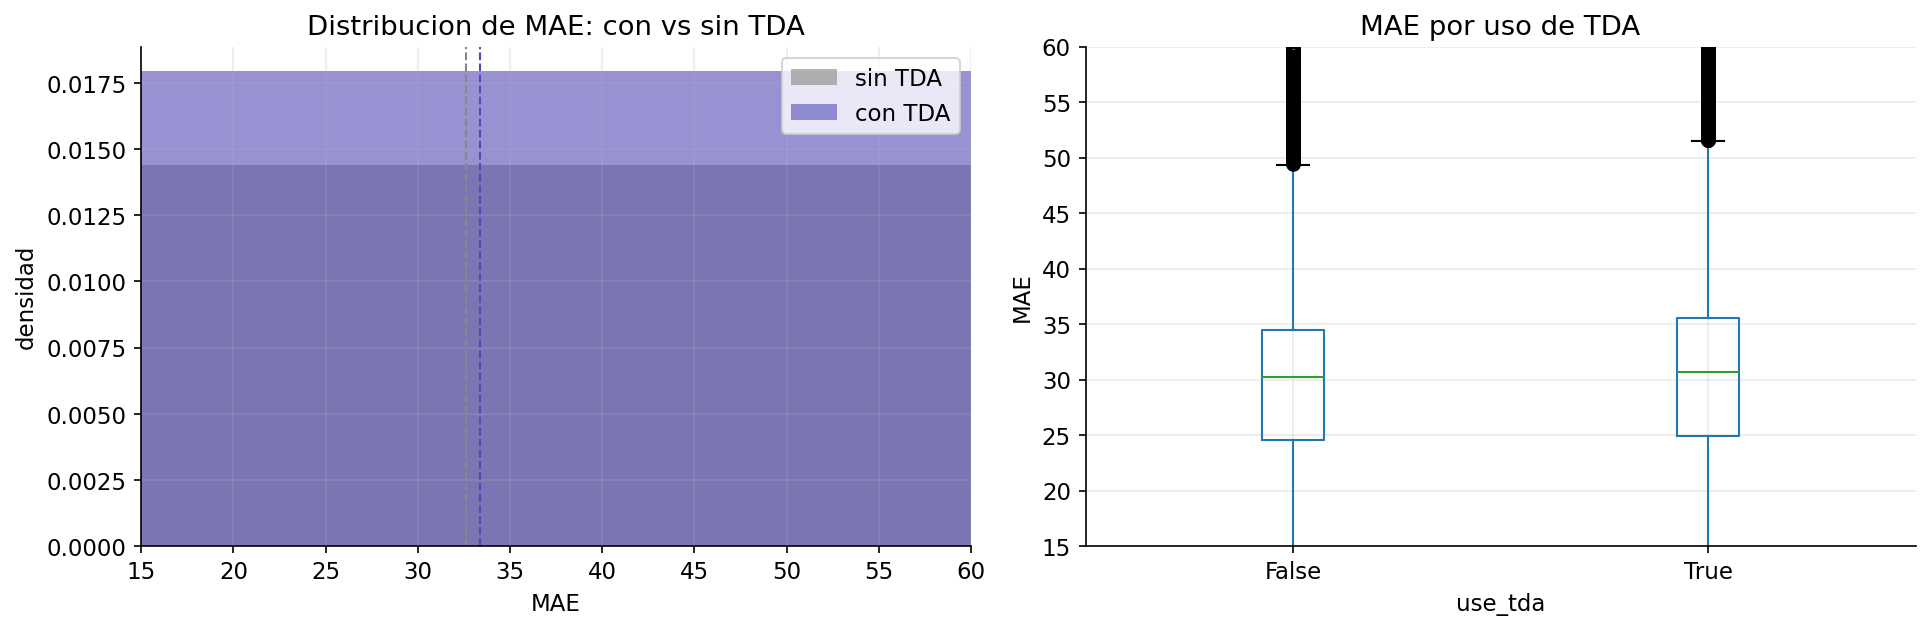
\includegraphics[width=\textwidth]{fig_efecto_tda.png}
    \caption{Efecto del TDA.}
  \end{subfigure}\hfill
  \begin{subfigure}{0.48\textwidth}
    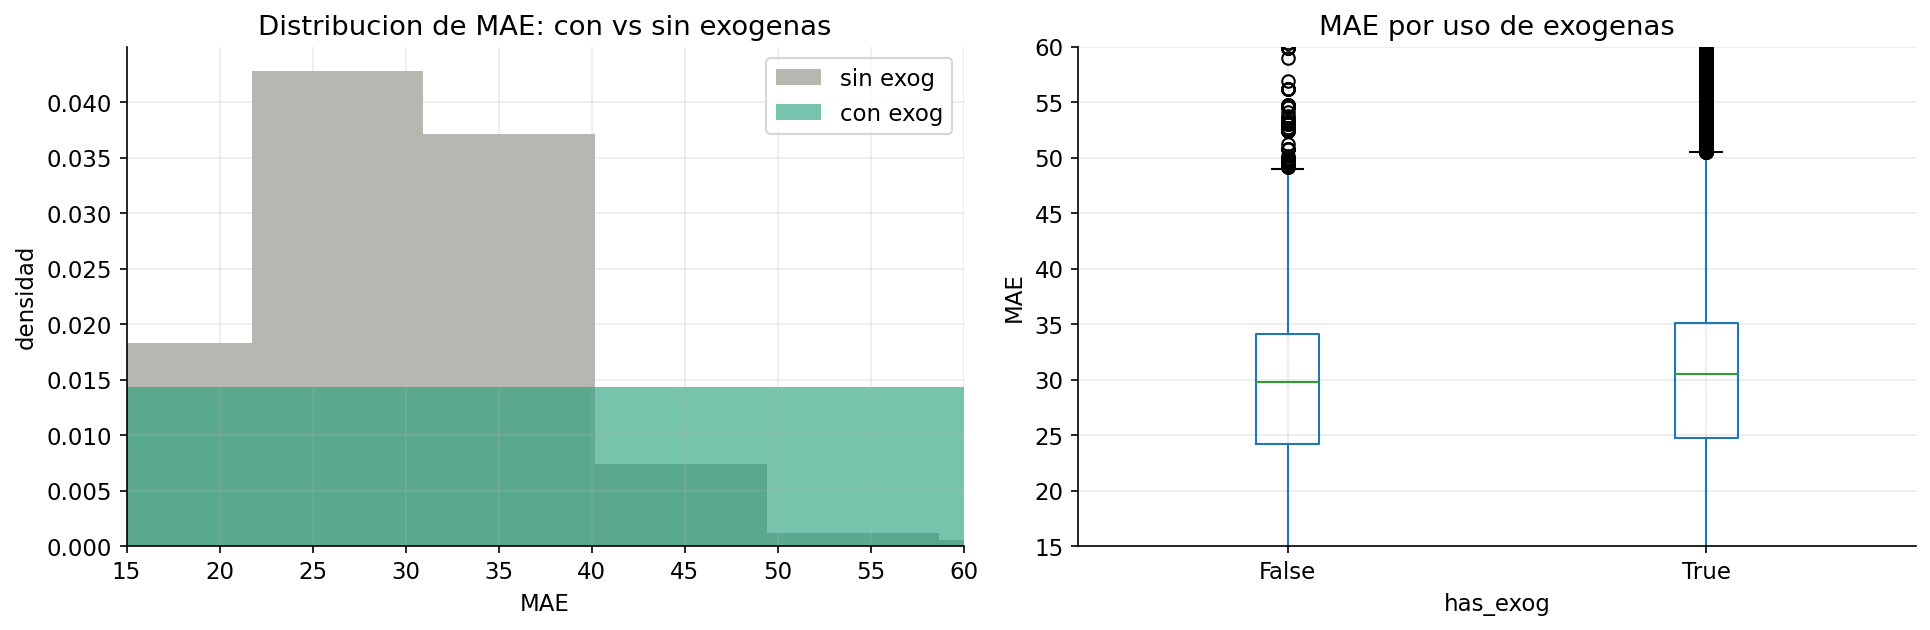
\includegraphics[width=\textwidth]{fig_efecto_exog.png}
    \caption{Efecto de las exógenas.}
  \end{subfigure}
  \caption{Distribución del MAE por fold con y sin cada factor. En ambos casos las
  distribuciones se solapan casi por completo.}
  \label{fig:efectos}
\end{figure}

\begin{figure}[H]
  \centering
  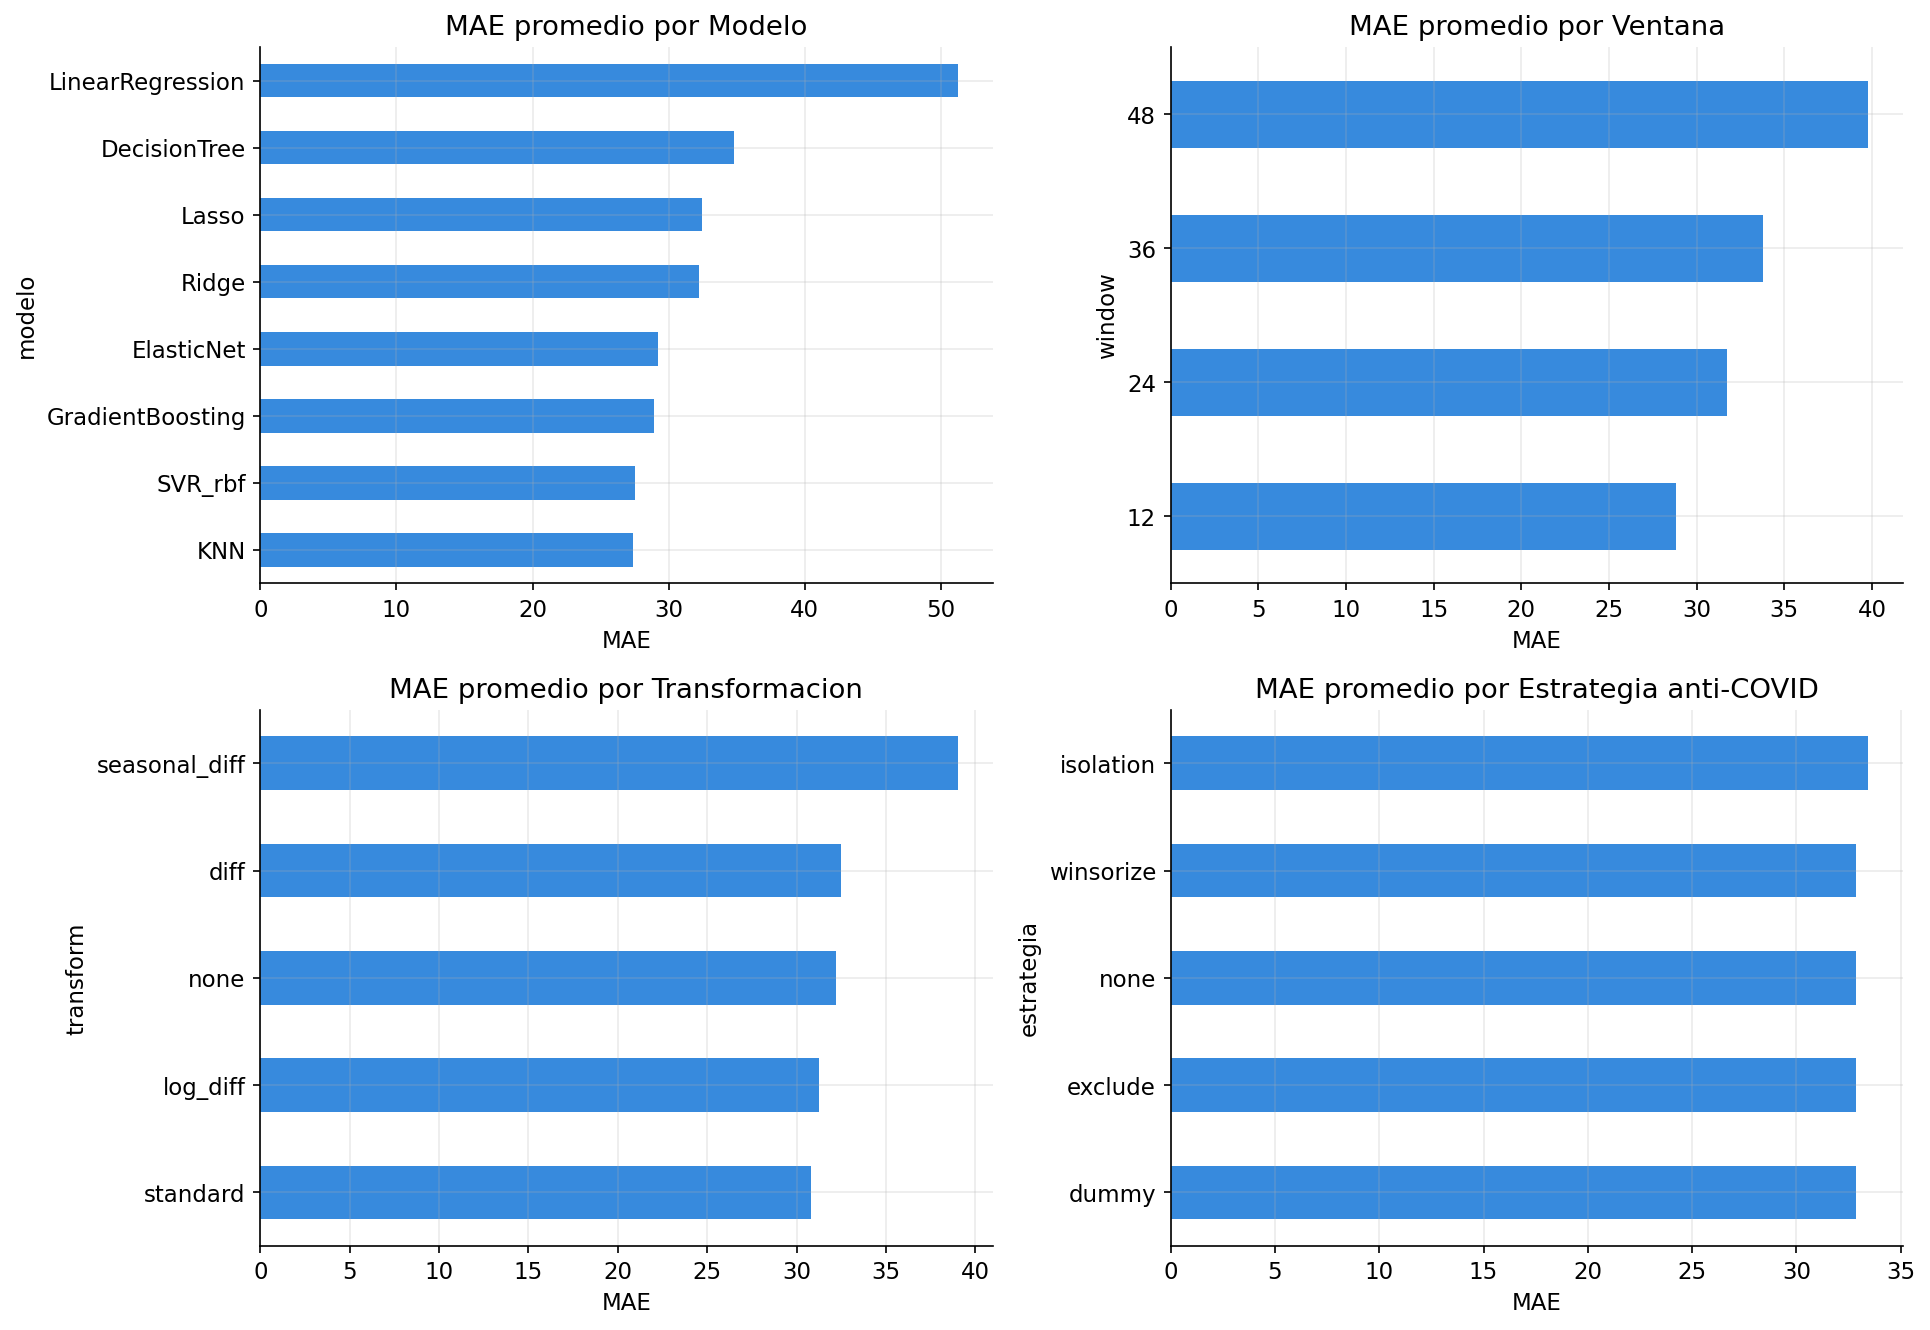
\includegraphics[width=0.92\textwidth]{fig_factores_individuales.png}
  \caption{Influencia de cada factor del pipeline sobre el MAE: el modelo y la
  longitud de ventana dominan; el TDA es marginal.}
  \label{fig:factores}
\end{figure}

\subsection{Desempeño final en el conjunto de prueba (2022 en adelante)}
Los modelos ganadores (seleccionados sin tocar el conjunto de prueba) se
evaluaron sobre el periodo de prueba. La Tabla~\ref{tab:final} y la
Figura~\ref{fig:testcomb} resumen el resultado: el mejor modelo es un Ridge sin
exógenas ni TDA (ventana 12, transformación log\_diff), con MAE $=29.79$ y
$R^2=0.469$. La variante con exógenas (un Lasso) queda prácticamente empatada, y
ninguna de las configuraciones ganadoras emplea TDA.

\begin{table}[H]
  \centering
  \caption{Métricas en el conjunto de prueba (enero 2022 en adelante) de las
  configuraciones finales.}
  \label{tab:final}
  \small
  \begin{tabular}{lrrrr}
    \toprule
    Modelo & MAE & RMSE & MAPE (\%) & $R^2$ \\
    \midrule
    Mejor sin exógenas (Ridge, log\_diff) & 29.79 & 37.09 & 21.52 & 0.469 \\
    Mejor con exógenas (Lasso, ppi\_fertilizers) & 30.00 & 37.79 & 21.79 & 0.449 \\
    Mejor estadístico en validación cruzada & 31.94 & 41.03 & 21.78 & 0.350 \\
    \bottomrule
  \end{tabular}
\end{table}

\begin{figure}[H]
  \centering
  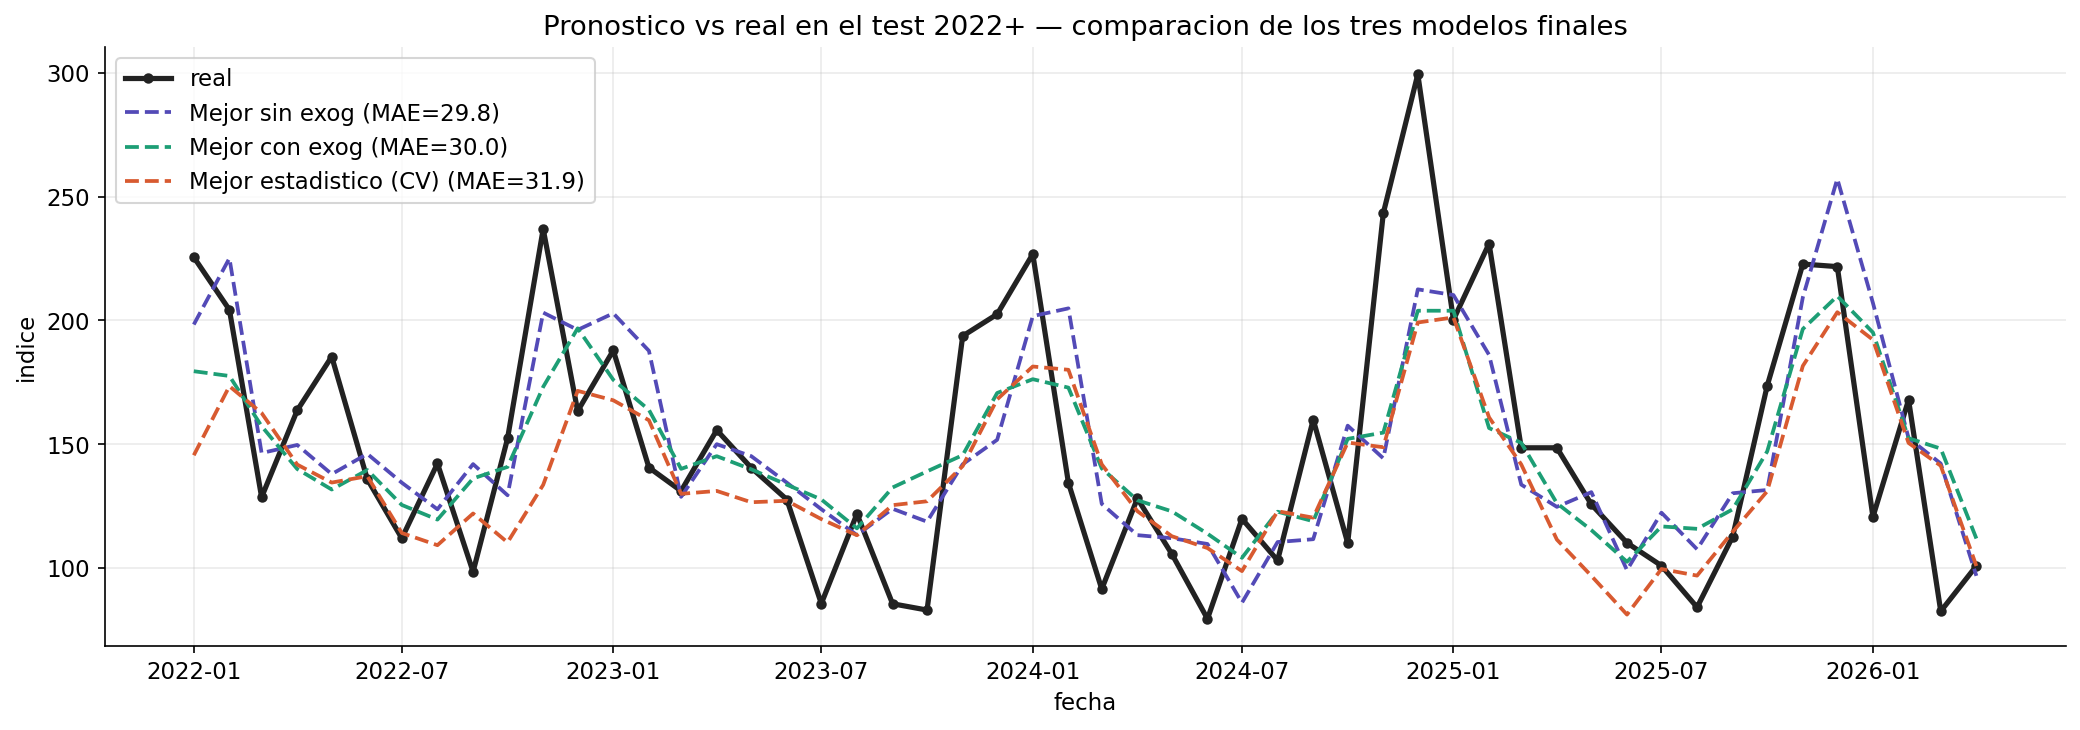
\includegraphics[width=0.95\textwidth]{fig_forecast_vs_test_combinado.png}
  \caption{Comparación de predicciones contra los valores reales en el conjunto
  de prueba 2022 en adelante para los tres modelos finales.}
  \label{fig:testcomb}
\end{figure}

\begin{figure}[H]
  \centering
  \begin{subfigure}{0.49\textwidth}
    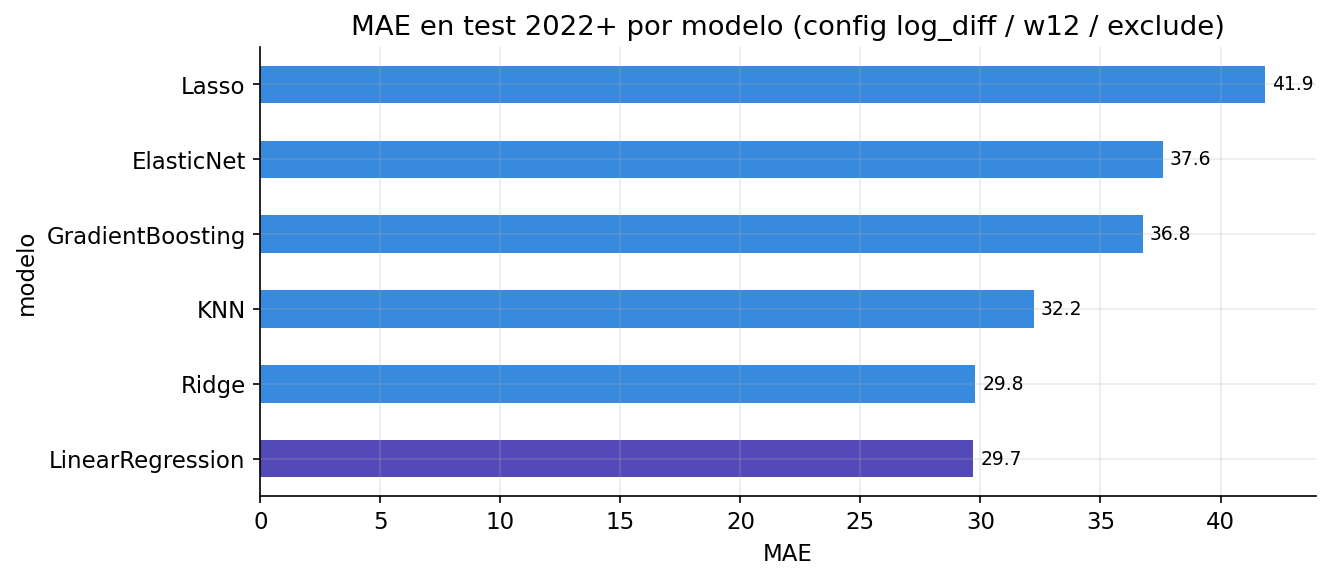
\includegraphics[width=\textwidth]{fig_ranking_test.png}
    \caption{Ranking de modelos en prueba.}
  \end{subfigure}\hfill
  \begin{subfigure}{0.49\textwidth}
    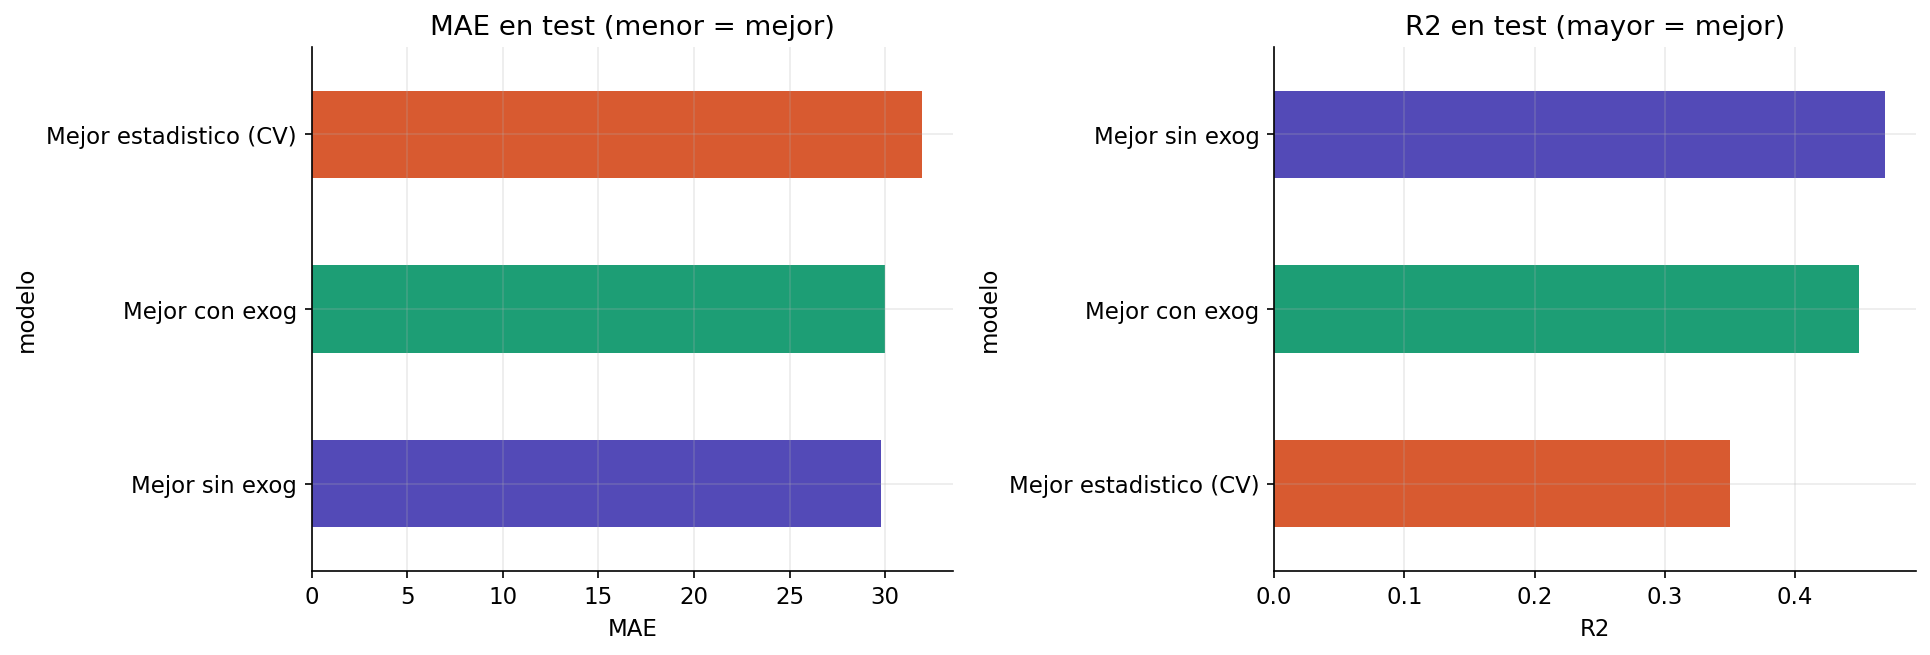
\includegraphics[width=\textwidth]{fig_forecast_metricas_barras.png}
    \caption{Métricas comparadas.}
  \end{subfigure}
  \caption{Ranking y métricas de las configuraciones evaluadas en el conjunto de
  prueba.}
  \label{fig:ranking}
\end{figure}

\subsection{Comparación dirigida RF y SARIMA con y sin TDA}
\label{sec:rfsarima}
Replicando el contraste sugerido en el enunciado sobre la ventana reciente
(Tabla~\ref{tab:rfsarima}), se observa el mismo patrón: SARIMA domina ampliamente
a los modelos basados en Random Forest, y añadir TDA prácticamente no cambia el
resultado (mejora marginal de $+0.25\%$ en RF y un leve deterioro en SARIMA).

\begin{table}[H]
  \centering
  \caption{Comparación dirigida sobre la ventana reciente (2025 a 2026). La
  columna de mejora se mide respecto al RF base.}
  \label{tab:rfsarima}
  \small
  \begin{tabular}{lrrrr}
    \toprule
    Modelo & MAE & RMSE & $R^2$ & Mejora vs.\ RF base \\
    \midrule
    RF Sin TDA   & 41.19 & 52.10 & $-0.131$ & (base) \\
    RF + TDA     & 41.09 & 52.04 & $-0.128$ & $+0.25\%$ \\
    SARIMA       & 29.42 & 36.11 & $0.457$ & $+28.58\%$ \\
    SARIMA + TDA & 30.60 & 36.45 & $0.446$ & $+25.71\%$ \\
    \bottomrule
  \end{tabular}
\end{table}

\subsection{Predicciones futuras}
La Tabla~\ref{tab:forecast} presenta el pronóstico directo a 12 meses
(mayo 2026 a abril 2027) de los cuatro modelos. Todos capturan el repunte
estacional de otoño, aunque RF y SARIMA discrepan en la magnitud del pico
(por ejemplo, octubre 2026). Una vez más, las variantes con y sin TDA son casi
indistinguibles.

\begin{table}[H]
  \centering
  \caption{Pronóstico del índice WPUSI01102B a 12 meses.}
  \label{tab:forecast}
  \small
  \begin{tabular}{lrrrr}
    \toprule
    Mes & RF Sin TDA & RF + TDA & SARIMA & SARIMA + TDA \\
    \midrule
    May 2026 & 111.10 & 109.85 & 124.98 & 125.47 \\
    Jun 2026 & 114.72 & 113.77 & 116.08 & 116.38 \\
    Jul 2026 & 110.50 & 110.71 & 114.16 & 114.47 \\
    Ago 2026 & 113.12 & 112.90 & 116.60 & 116.93 \\
    Sep 2026 & 125.79 & 125.98 & 129.43 & 130.06 \\
    Oct 2026 & 218.96 & 220.61 & 139.75 & 140.19 \\
    Nov 2026 & 177.47 & 177.19 & 208.96 & 207.59 \\
    Dic 2026 & 164.59 & 164.02 & 218.88 & 217.77 \\
    Ene 2027 & 154.82 & 151.40 & 192.14 & 191.31 \\
    Feb 2027 & 158.91 & 157.91 & 186.08 & 185.75 \\
    Mar 2027 & 134.59 & 133.92 & 135.98 & 136.09 \\
    Abr 2027 & 111.40 & 112.51 & 148.75 & 149.36 \\
    \bottomrule
  \end{tabular}
\end{table}

\subsection{Optimización de hiperparámetros (Optuna)}
El barrido factorial completo de la Sección anterior recorre cerca de 19\,200
combinaciones por fold y, aunque es ideal para inferencia estadística (permite
medir el efecto marginal de cada factor con pruebas pareadas), tiene un costo
computacional alto y crece de forma multiplicativa con cada nuevo factor o nivel.
Por ello se incorporó además una búsqueda con Optuna sobre el conjunto de
validación, que aproxima la mejor configuración mediante muestreo bayesiano sin
evaluar exhaustivamente toda la malla.

Esto justifica su uso en dos escenarios prácticos: cuando se disponga de más
datos o más factores (donde el barrido marginal completo se vuelve inviable por
el tiempo de cómputo) y cuando no se quiera o no se pueda costear un
entrenamiento tan largo. Optuna alcanza configuraciones competitivas en una
fracción de las evaluaciones, lo que lo hace adecuado para un entorno industrial
donde el modelo debe re-entrenarse con frecuencia y bajo restricciones de tiempo.
La Figura~\ref{fig:optuna} muestra la convergencia y la importancia de
hiperparámetros de esta búsqueda.

\begin{figure}[H]
  \centering
  \begin{subfigure}{0.55\textwidth}
    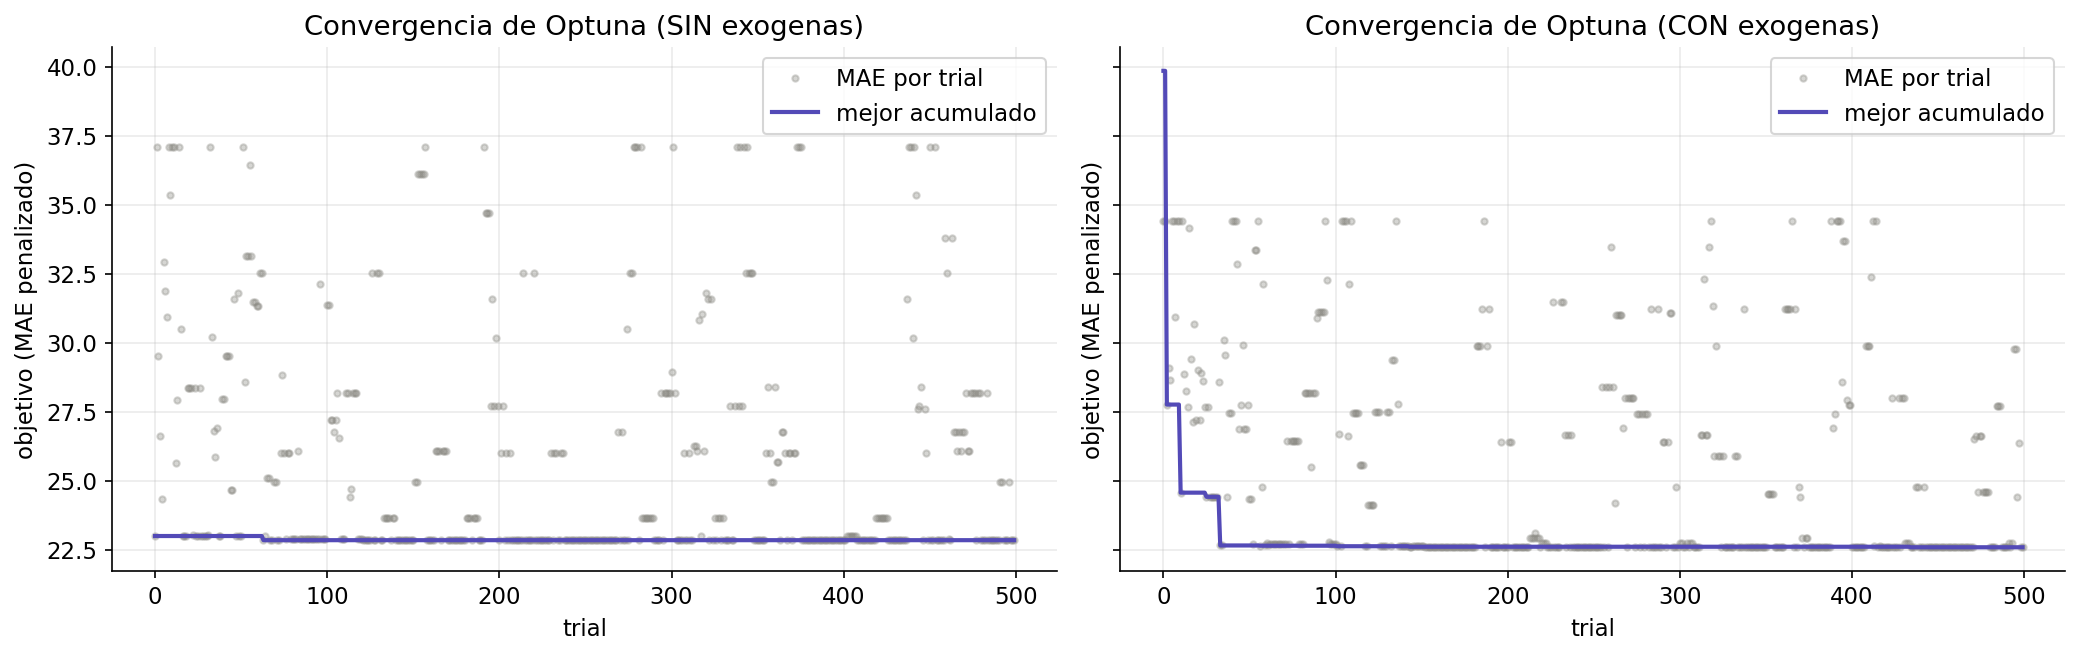
\includegraphics[width=\textwidth]{fig_optuna_convergencia.png}
    \caption{Convergencia.}
  \end{subfigure}\hfill
  \begin{subfigure}{0.43\textwidth}
    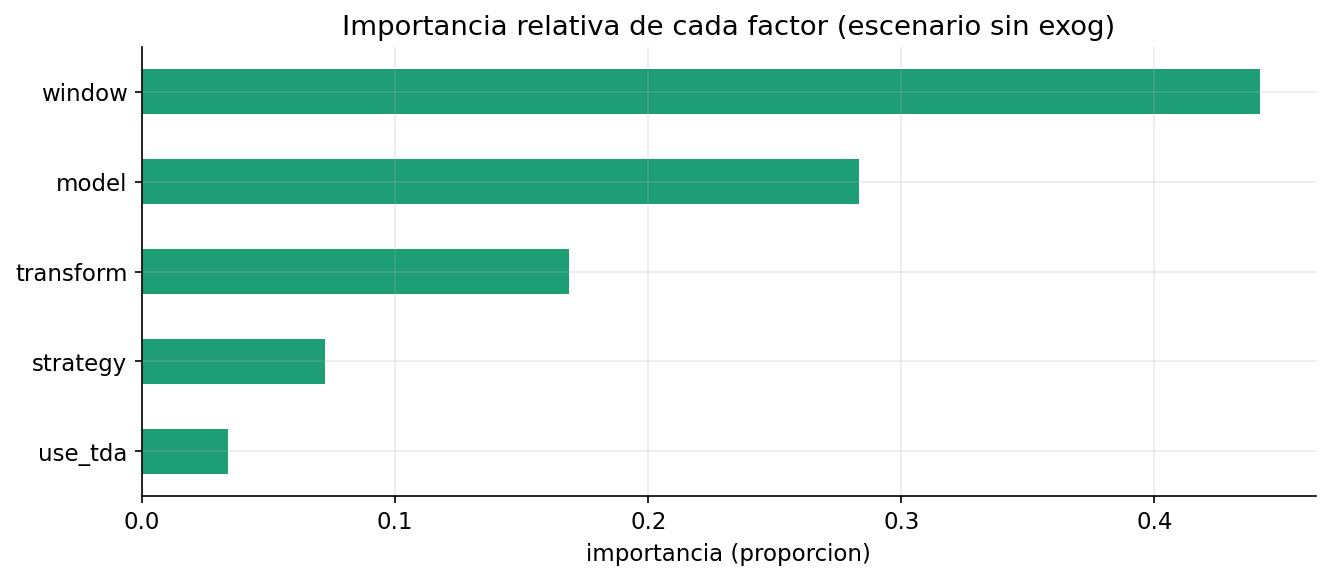
\includegraphics[width=\textwidth]{fig_optuna_importancia.png}
    \caption{Importancia de hiperparámetros.}
  \end{subfigure}
  \caption{Optimización con Optuna de la configuración del pipeline.}
  \label{fig:optuna}
\end{figure}

% ==================================================================
\section{Discusión}
% ==================================================================
La evidencia es consistente a lo largo de las tres líneas de análisis (factorial
en validación cruzada, evaluación en prueba y comparación dirigida RF y SARIMA) y
apunta en la misma dirección: para esta serie el TDA no aporta señal predictiva
útil. Aunque las pruebas detectan un efecto significativo (consecuencia del
tamaño muestral de decenas de miles de pares), el tamaño de efecto de Cliff
($0.047$) es despreciable y el signo es contraproducente.

Una explicación plausible es que la estacionalidad de la serie, el rasgo que la
homología persistente $H_1$ pretende capturar, ya está plenamente codificada en
los retardos de la ventana, que todos los modelos reciben. El TDA, por tanto,
agrega redundancia y dimensionalidad (8 columnas extra) sin información nueva, lo
que perjudica especialmente a los modelos lineales regularizados. El resultado
para las exógenas es análogo: añaden ruido más que señal en el horizonte $t{+}1$.

Hallazgos secundarios: el modelo y la longitud de ventana son los factores
dominantes, donde ventanas largas ($w=48$) degradan mucho el error ($+11.4$ MAE);
la transformación log\_diff es la mejor y seasonal\_diff la peor; y SARIMA es un
baseline muy competitivo, difícil de superar por los regresores supervisados.

% ==================================================================
\section{Conclusiones}
% ==================================================================

\subsection*{Resumen de hallazgos}
\begin{itemize}[noitemsep]
  \item El mejor modelo final es Ridge sin TDA ni exógenas (MAE $=29.79$,
        $R^2=0.469$ en prueba).
  \item El efecto del TDA es estadísticamente detectable pero de magnitud
        insignificante ($\delta=0.047$) y ligeramente adverso ($+0.76$ MAE).
  \item Las exógenas tampoco ayudan en $t{+}1$ ($+2.49$ MAE).
  \item SARIMA supera a los modelos tipo RF por un amplio margen (cerca de 29\%).
\end{itemize}

\subsection*{Conclusiones}
Para el forecasting del precio de berries (WPUSI01102B), no se justifica el uso de
TDA: el costo computacional adicional de la homología persistente no se traduce en
mejor precisión, porque la información topológica ya está implícita en los
retardos. Un modelo lineal regularizado sencillo sobre la serie diferenciada en
logaritmos, o bien un SARIMA estacional, ofrecen el mejor compromiso entre
precisión y simplicidad.

\subsection*{Trabajo futuro}
\begin{itemize}[noitemsep]
  \item Evaluar TDA en horizontes más largos ($h>1$) o en clasificación de
        regímenes y anomalías, donde la forma global podría ser más informativa
        que para regresión a un paso.
  \item Explorar otras vectorizaciones topológicas (persistence images,
        landscapes) y embeddings multivariados que incorporen exógenas.
  \item Probar modelos secuenciales (LSTM o Temporal CNN) y combinaciones de
        SARIMA con regresores.
  \item Ampliar el conjunto exógeno (clima, índices de producción agrícola) con
        retardos seleccionados por causalidad.
\end{itemize}

\vspace{1em}
\noindent\rule{\textwidth}{0.4pt}\\[2pt]
\small
Reproducibilidad. Repositorio:
\url{https://github.com/xGonks/berry-price-tda}. Código en src/berry\_price\_tda/
y scripts/. Todo el flujo se orquesta con un Makefile: make data y make exog
descargan la serie y las exógenas, make optuna y make optuna-exog ejecutan la
búsqueda de hiperparámetros, make experiment corre el barrido factorial completo
con su análisis estadístico, y make full encadena el proceso de principio a fin
(datos, exógenas, Optuna, factorial, análisis). Resultados en data/processed/ y
figuras en reports/figures/.

\end{document}
